This section deals with the new SmartRobotinoMPSDocking component. The new docking algorithm is discussed in this chapter, including the advantages and disadvantages of the new approach.

\subsubsection{Overview}

The new docking approach is much more lightweight than the previous one from 2017.

\begin{figure}[h]
\centering
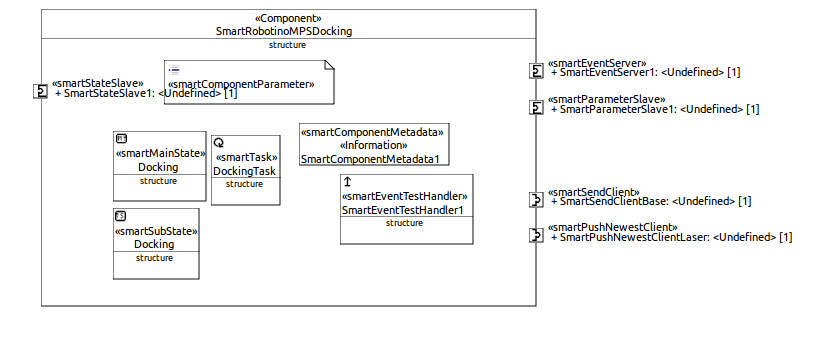
\includegraphics[scale=0.65]{pic/dockingComponent.png}
\caption{Model of the new Docking Component }
\label{fig:i_overview}
\end{figure}

The component consists mainly of one task (e.g. DockingTask), which just performs the docking to the corners of a MPS station, provided by the detection component.

\subsubsection{Previous Version 2017}

The docking procedure of the former team was part of the SmartMPSDockingRoboCup component, which combined the detection task with the docking task.
The docking algorithm is implemented in a very incomprehensible way and also provides random docking results. Therefore, the team of 2018 implemented a completely new docking component, which is lightweight, easy to understand and simple to optimize.

\subsubsection{New Version 2018}

For the new docking approach, the two corners of the target MPS station are enough information. The docking task performs the following procedure:

\begin{enumerate}
\item Turn towards the target MPS station
\item Calculate the angle between robot and MPS station
\item Turn left or right until angle of robot to station is around 90 degrees
\item Drive towards the middle of the MPS station, while angle to station is kept to around 90 degrees
\end{enumerate}

The calculation of the angle between robot and the target MPS station is described in the next paragraph.

\subsubsection{Calculation of the angle between robot and MPS}

The corners of the target MPS station assemble a vector (e.g. stationVector). The robot has also a direction vector assigned to it, which is always pointing in the facing direction of the robot (e.g. roboDirectionVector). For the calculation of the angle between the robot and the MPS, the well-known formula of the dot product of the two vectors divided by the length of the both vectors is used. To get always the acute angle of the vectors, the absolute value of the dot product is used. 

\begin{equation}
\cos(\phi) = \frac{ \vert \overrightarrow{roboDirectionVector} \circ \overrightarrow{stationVector} \vert} { \vert \overrightarrow{roboDirectionVector}  \vert  \cdot \vert \overrightarrow{stationVector}  \vert}
\end{equation}

\begin{equation}
\phi = \cos ^{ - 1} \left( \frac{ \vert \overrightarrow{roboDirectionVector} \circ \overrightarrow{stationVector} \vert} { \vert \overrightarrow{roboDirectionVector}  \vert  \cdot \vert \overrightarrow{stationVector}  \vert} \right)
\end{equation}


This approach only works, if the robot somehow faces the target MPS machine. Thats why the robot turns towards the target MPS station, before calculating the angle (robot - station). 


\subsubsection{Optimizations}
Several optimizations can be done at the RoboCup. 

\begin{enumerate}
\item Increase the speed of turning
\item Increase the speed of driving towards the center of the MPS station
\item Introduce a minimal and maximal distance to the MPS station (e.g. 1 meter), to stay in range for the ALVAR Tag detection
\end{enumerate}
 

\subsubsection{Summary}
The new docking component works very well. The component docks successfully at all docking situations (MPS stands 0, 45, 90, 135, 180, 225, 270, and 315 degrees to the robot).
The approach is easy to extend and to optimize. It was not possible to reuse the old component smartMPSDockingRobocup, which combined detection with docking. It would have been too time consuming, finding all the bugs in the overcomplicated component. 
